\section{Literature Review}

\subsection{Existing solutions}

	\subsubsection{Group Chat-Based Systems (Current Solution at VGU)}
		Currently, many educational institutions, including VGU, rely on informal systems like social media group chats (e.g., Facebook or WhatsApp groups) for raising support tickets and contacting staff. While these systems are easy to set up and require minimal resources, they suffer from significant limitations:
		
		\begin{itemize}
			\item[-] \textbf{Lack of Structure}: The conversation threads are disorganized, making it hard to track specific issues or prioritize them.
			
			\item[-] \textbf{Absence of Accountability}: There’s no formal ticketing system, leading to delays in responses and no mechanism to track whether an issue has been resolved.
			
			\item[-] \textbf{Inadequate Historical Data}: It's difficult to retrieve past conversations or analyze data to improve service.
			
			\item[-] \textbf{Lack of Privacy}: Group chats often expose personal information to all participants, which may raise privacy concerns.
		\end{itemize}
		
		
		\subsubsection{Existing University Ticketing Systems}
		Several universities have adopted formal ticket management systems for handling student support services. These systems are often integrated into larger university management platforms or custom-built web applications. Common examples include:
		
		\begin{longtable}{{|l|m{6cm}|m{6cm}|}} 
			\hline
			\textbf{Systems} & \textbf{Features} &\textbf{Limitations}\\ \hline
			\endhead
			JIRA Service Management 
			& Offers customizable workflows, automated prioritization, and detailed issue tracking.
			& Too complex for university needs, expensive, and difficult to adapt without major customization.
			\\ \hline
			Freshdesk 
			& Supports ticket management, multi-channel communication, and agent collaboration. 
			& Feature-heavy and expensive for universities; lacks educational-specific tools.
			\\ \hline
			Zendesk 
			&  Provides email, live chat, and ticketing, with automation and analytics. 
			& Geared towards businesses; lacks flexibility for diverse student needs and real-time communication.
			\\ \hline
			OSTicket
			& Open-source, customizable, with email-based ticketing and status tracking.
			& Requires customization for universities, not intuitive for non-technical users, lacks real-time communication.
			\\ \hline
			
			\caption{Existing University Ticketing Systems} % needs to go inside longtable environment
			\label{tab:existing-ticket-sys}
		\end{longtable}
		
	\subsubsection{Limitations of Existing Solutions in the University Context}
	
		\begin{itemize}
			\item[-] \textbf{Complexity}: Many existing solutions are designed for enterprise environments and are not tailored to the unique requirements of universities.
			\item[-] \textbf{Lack of Customization}: Solutions like JIRA and Zendesk require extensive customization to meet university-specific needs, such as handling dormitory issues or academic support tickets.
			\item[-] \textbf{Cost}: Proprietary solutions can be expensive, making them less viable for universities with limited IT budgets.
			\item[-]\textbf{ Lack of Real-Time Communication}: Most solutions offer asynchronous communication through email or message boards but do not provide real-time chat, which is essential for time-sensitive student support.
		\end{itemize}

\subsection{Technology Review}

	\subsubsection{Frontend: ReactJS, Material UI, Vite}
	
	
%	\begin{wrapfigure}{l}{0.25\textwidth}
%		
\includegraphics[width=0.5\linewidth]{graphics/React_Logo_SVG.png} 
%		\caption{React}
%		\label{fig:react}
%	\end{wrapfigure}
	
	  \begin{tabular}{ @{} m{0.25\textwidth} m{0.7\textwidth} @{} }
		\begin{minipage}{\linewidth}
			\centering
			
\includegraphics[width=0.6\linewidth]{graphics/React_Logo_SVG.png}
			\captionof{figure}{React Logo}
			\label{fig:react}
		\end{minipage}
		&
		\begin{minipage}{\linewidth}
			\textbf{React} is a popular JavaScript library for building user interfaces, which provides a fast, scalable, and modular way to develop the frontend of web applications \cite{react}. Its component-based architecture allows for reusability and efficient state management using hooks like \textbf{\texttt{useState()}} and \textbf{\texttt{useEffect()}}. This enables a responsive and dynamic user experience, ideal for handling real-time ticket updates.
		\end{minipage}
	\end{tabular}
	
	\vspace*{1cm}
	
	\begin{lstlisting}[language=Javascript, caption=Example of a React component]
		const Profile = () => {
			
			return (
				<MainCard title="Personal Information">
					<Grid container spacing={gridSpacing}>
				
						<Grid item xs={12} sm={6}>
							<ProfileCard />
						</Grid>
					
						<Grid item xs={12} sm={6}>
							<SchoolDetailsCard/>
						</Grid>
				
					</Grid>
				</MainCard>
			);
		}
		
		export default Profile;
	\end{lstlisting}
	
	
	 \begin{tabular}{ @{} m{0.7\textwidth} m{0.25\textwidth} @{} }
		\begin{minipage}{\linewidth}
			\textbf{Material UI} is a React-based UI component library that implements Google’s Material Design principles. Material UI ensures that the frontend is both visually appealing and functionally intuitive. Pre-built components like buttons, forms, and dialogs accelerate development while maintaining consistency in design. \cite{material-ui}
		\end{minipage}
		&
		\begin{minipage}{\linewidth}
				\centering
			
\includegraphics[width=0.6\linewidth]{graphics/material-ui-480.png}
			\captionof{figure}{Material UI Logo}
			\label{fig:material-ui}

		\end{minipage}
	\end{tabular}
	
	\vspace*{0.5 cm}
	
	\begin{tabular}{ @{} m{0.25\textwidth} m{0.7\textwidth} @{} }
		\begin{minipage}{\linewidth}
			\centering
			
\includegraphics[width=0.5\linewidth]{graphics/vite.png}
			\captionof{figure}{Vite Logo}
			\label{fig:vite}
		\end{minipage}
		&
		\begin{minipage}{\linewidth}
			\textbf{Vite}, a modern frontend build tool that offers faster development speed compared to older tools like Webpack. Vite optimizes the build process for React applications by providing instant hot module replacement (HMR), which is useful for a smooth developer experience during iterative development cycles. \cite{vite}
		\end{minipage}
	\end{tabular}
	\vspace*{0.5 cm}
	
	
	\subsubsection{Backend: NodeJS, ExpressJS, SocketIO}
	
	\vspace*{0.5 cm}
	\begin{tabular}{ @{} m{0.25\textwidth} m{0.7\textwidth} @{} }
		\begin{minipage}{\linewidth}
			\centering
			
\includegraphics[width=0.5\linewidth]{graphics/nodejs.png}
			\captionof{figure}{NodeJS Logo}
			\label{fig:nodejs}
		\end{minipage}
		&
		\begin{minipage}{\linewidth}
			\textbf{NodeJS} is a runtime that enables JavaScript to be used for server-side scripting, making it possible to use a single language (JavaScript) throughout the stack. NodeJS is non-blocking and event-driven, making it ideal for handling I/O-heavy tasks like managing support ticket requests in real time.
		\end{minipage}
	\end{tabular}
	
	\vspace*{0.5cm}
	
	\begin{tabular}{ @{} m{0.7\textwidth} m{0.25\textwidth} @{} }
		\begin{minipage}{\linewidth}
			\textbf{ExpressJS} is a minimalist web framework for NodeJS, Express simplifies routing, middleware management, and API handling. It serves as the backbone of the server, processing requests from the frontend, interacting with the database, and managing the business logic.
		\end{minipage}
		&
		\begin{minipage}{\linewidth}
			\centering
			
\includegraphics[width=0.8\linewidth]{graphics/expressjs.png}
			\captionof{figure}{Expressjs Logo}
			\label{fig:expressjs}
			
		\end{minipage}
	\end{tabular}
	
	\vspace*{0.5cm}
	\begin{tabular}{ @{} m{0.25\textwidth} m{0.7\textwidth} @{} }
		\begin{minipage}{\linewidth}
			\centering
			
\includegraphics[width=0.5\linewidth]{graphics/socket-io.512x512.png}
			\captionof{figure}{SocketIO Logo}
			\label{fig:socketio}
		\end{minipage}
		&
		\begin{minipage}{\linewidth}
			\textbf{SocketIO} is a JavaScript library that enables real-time, bidirectional communication between clients and servers. SocketIO is used to implement features such as real-time messaging between students and staff, making the system more interactive and responsive. \cite{socketio}
		\end{minipage}
	\end{tabular}
	
	
	\subsubsection{Authentication: JWT, Redis}
	\vspace*{0.5cm}
	\begin{tabular}{ @{} m{0.25\textwidth} m{0.7\textwidth} @{} }
		\begin{minipage}{\linewidth}
			\centering
			
\includegraphics[width=0.5\linewidth]{graphics/jwt-logo.png}
			\captionof{figure}{JWT Logo}
			\label{fig:jwt }
		\end{minipage}
		&
		\begin{minipage}{\linewidth}
			JWT (JSON Web Tokens)is a token-based authentication system that provides secure stateless authentication for users. JWT is ideal for modern web applications because tokens can be stored on the client-side (in local storage or cookies) and are transmitted with each request, allowing for scalability.
		\end{minipage}
	\end{tabular}
	
	\begin{center}
		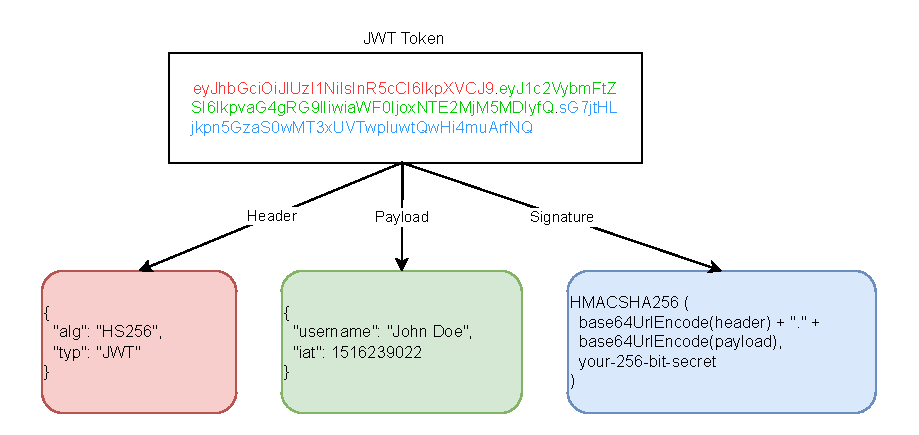
\includegraphics[width=1.1\columnwidth]{graphics/jwt-explained.pdf}
	\end{center}
	
	
	
	
			